\chapter{Ambiente di sviluppo}

In questo capitolo saranno discusse le funzionalità e le possibilità offerte dal progetto in questione a favore del programmatore, nonché i vantaggi e le migliorie apportate nel processo di sviluppo.

La difficoltà principale che un programmatore si trova ad affrontare nell'intraprendere un percorso di apprendimento della programmazione embedded consiste nel ritrovarsi in un mondo completamente diverso di gestione del software e ambienti di sviluppo. Vi è poi l'assoluta differenza del processo di programmazione e debug da un comune applicativo per calcolatore.

Sebbene l'approccio a una nuova piattaforma hardware con differenti specifiche e funzionalità e, spesso, con un \textit{instruction set} limitato e non famigliare possa sembrare un ostacolo impegnativo, nella realtà, grazie a strumenti quali compilatori come \textit{gcc} e \textit{rustc}, è possibile scrivere notevoli porzioni di codice completamente indipendenti dall'architettura del dispositivo finale.

La difficoltà principale per lo sviluppatore nell'approcciarsi allo sviluppo di una piattaforma embedded è di fatto l'adattarsi ad un nuovo ambiente e strumenti spesso proprietari e male o per nulla documentati.

Un'ulteriore difficoltà che limita l'accesso di nuovi sviluppatori verso il mondo embedded è la necessità di strumenti proprietari e costosi per programmare e \textit{debuggare} hardware, oltre al costo fisico di schede per la prototipazione.

Questi fattori sopra elencati hanno permesso alla società \textit{Arduino~s.r.l.} di entrare nel mercato dei dispositivi embedded mirando ad un pubblico inesperto e desideroso di approcciare una nuova pratica\cite{site:arduino-about}.

L'ecosistema Arduino è la scelta adottata dalla maggior parte di hobbisti e corsi di introduzione al mondo dell'elettronica digitale, motivati dalla dimensione della \textit{community}\footnote{Supporto di altri utenti fornito per mezzo di forum e mezzi anche non gestiti dall'azienda produttrice}, dal supporto, dagli strumenti sviluppati compatibili e semplici e dalla quantità di librerie \textit{open source} disponibili.

Non vi è dubbio sulla versatilità e la facilità di apprendimento della programmazione embedded AVR tramite la piattaforma.

Date le motivazioni e l'obiettivo dell'azienda d'Ivrea, è possibile osservare come la piattaforma e gli strumenti software non siano ottimali per uno sviluppo professionale o più complesso e ottimizzato.

\begin{figure}
    \centering
    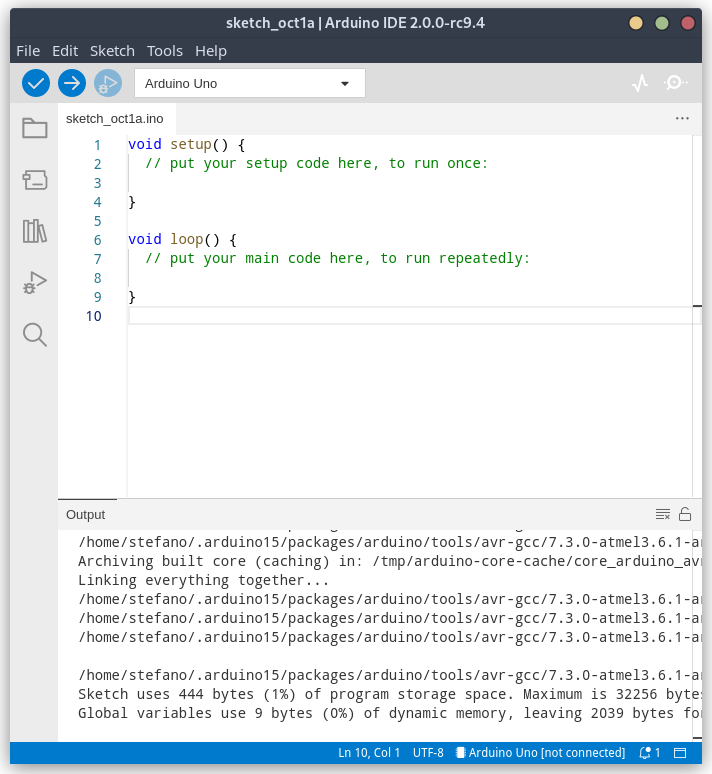
\includegraphics[width=.6\textwidth]{arduino-ide.png}
    \caption[Immagine del software Arduino IDE v2]{Finestra di programmazione dell'ambiente di sviluppo Arduino IDE v2}\label{fig:arduino-ide}
\end{figure}

Come è possibile osservare l'ambiente di sviluppo \textit{Arduino IDE} mostrato in~\cref{fig:arduino-ide} presenta un insieme notevolmente limitato di funzioni e un'interfaccia fortemente semplificata. È però possibile osservare la presenza di un indicatore di debug: questo è solo disponibile con schede ARM a 32 bit più prestazionali. La funzionalità di debug non è presente sulle schede AVR.\@

Data l'assenza del \textit{debugger} per la piattaforma AVR, gli utenti sono obbligati all'utilizzo di logging tramite connessione seriale per analizzare il flusso del codice, pratica fortemente inefficiente per motivi prestazionali e per problemi di codifica dell'informazione.

L'utilizzo del server GDB sviluppato nel corso di questo elaborato garantirebbe nuove possibilità e efficienza, risultano però complesso e poco intuitivo in quanto dotato di sola interfaccia testuale come mostrato dalla~\cref{fig:gdb-cli}

\begin{figure}
    \centering
    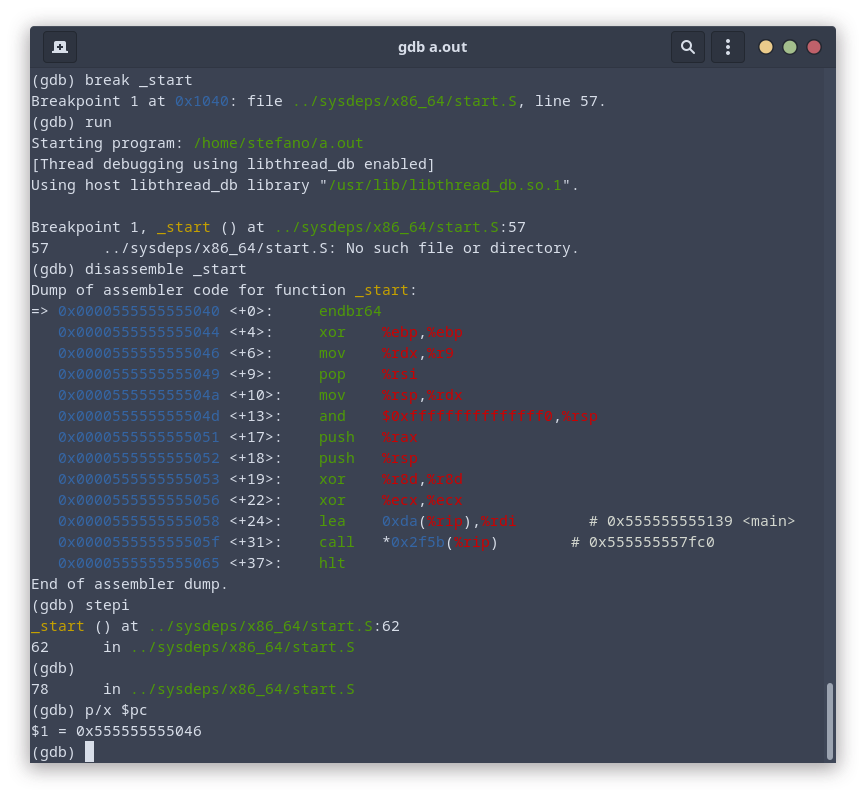
\includegraphics[width=.7\textwidth]{gdb-cli.png}
    \caption[]{Immagine di una sessione di debug da linea di comando}\label{fig:gdb-cli}
\end{figure}

Risulta quindi necessario sviluppare un insieme di strumenti che possano essere integrati nella maggior parte degli ambienti di sviluppo senza difficoltà, permettendo così di superare una delle limitazioni sopra descritte, ovvero la difficoltà di adottare un ambiente di sviluppo nuovo e mal documentato, permettendo l'utilizzo di una piattaforma nota e configurabile.

\section{CMAKE}\label{s:cmake}

Al fine di rendere la compilazione una procedura universale e generica è stato deciso l'utilizzo di un software di automazione del processo di compilazione altamente integrabile. Tale software è \textit{CMAKE}.

Esso permette di descrivere ad un livello più astratto gli obiettivi della compilazione e di impostare alcune variabili di configurazione per poi generare una procedura di compilazione in funzione delle librerie disponibili e delle caratteristiche dell'\textit{host}, semplificando la scrittura di codice interoperabile.

Inoltre, al fine di garantire interoperabilità tra ambienti di sviluppo, è stato deciso di affidare tutte le azioni di upload del codice a processi esterni che CMAKE permette di lanciare come degli obiettivi personalizzati.

L'integrazione con l'ambiente di sviluppo è invece affidata ad eventuali plugin per lo stesso o all'implementazione nativa del supporto per CMAKE.\@

Il~\cref{lst:cmake-target} mostra come un generico obiettivo di compilazione e programmazione viene descritto per poi essere tramutato in una procedura di compilazione.

È possibile notare come un singolo obiettivo per un dispositivo della piattaforma sia definito da tre distinti obiettivi concatenati e interdipendenti.

\noindent\begin{minipage}{\textwidth}
    \begin{lstlisting}[language=CMAKE, caption={Definizione di un target di compilazione e upload per un dispositivo AVR}, label=lst:cmake-target]
function(avrtarget targetName port)
    add_executable("${targetName}-elf" ${ARGN})
    target_link_options("${targetName}-elf" PUBLIC -Xlinker -T ${CMAKE_SOURCE_DIR}/cmake/linker/${MCU}.ld)
    add_custom_target(
        "${targetName}-bin" 
        COMMAND ${CMAKE_OBJCOPY} -O ihex -R .eeprom -R .fuse -R .lock -R .signature './${targetName}-elf' './${targetName}.hex';
        COMMAND ${CMAKE_OBJCOPY} -O ihex -j .eeprom './${targetName}-elf' './${targetName}.eeprom.hex';
        COMMAND ${CMAKE_SIZE} --mcu=${MCU} -C './${targetName}-elf';
        DEPENDS "${targetName}-elf"
    )
    add_custom_target(
        "${targetName}-upload"
        COMMAND python host_software/flash.py --port ${port} --flash './${targetName}.hex' --mcu ${MCU}
        USES_TERMINAL
        DEPENDS "${targetName}-bin"
    )
endfunction()

avrtarget(main main.c io.c)
target_link_libraries(main-elf rtt)
    \end{lstlisting}
\end{minipage}

In particolare sia \(main\) il nome generico assegnato all'obiettivo avr in sviluppo. La procedura di compilazione generata da CMAKE conterrà tre sotto obiettivi nominati
\begin{itemize}
    \item \textbf{main-elf}: obiettivo di compilazione effettivo dove il compilatore (\textit{avr-gcc}) verrà impiegato e genererà un file contenente codice eseguibile e informazioni di debug
    \item \textbf{main-bin}: obiettivo di utilità che estrarrà dal file \textit{build/main-elf} i file in formato \textit{ihex}\footnote{Intel Hexadecimal Format} per la programmazione delle memorie persistenti. Tali file sono una rappresentazione compressa del formato esadecimale\cite{site:ihex} e rappresentano le memorie bit per bit.
    \item \textbf{main-upload}: l'esecuzione di questo obiettivo esegue uno script che, dialogando con il server gdb, permette la scrittura della memoria flash e di conseguenza la programmazione senza uscire dalla modalità DebugWire.
\end{itemize}


\section{Ambiente di programmazione}

Per quanto riguarda l'ambiente di sviluppo, verrà commentata a seguire una configurazione di \textit{Visual Studio Code}.

La scelta di questo editor di testo è data dalla sua grande diffusione\cite{site:vscode-connect-2017} e dalla sua facilità di estensione tramite un sistema di plugin, con i quali diviene di fatto un ambiente di sviluppo integrato (IDE).

Inoltre, lo sviluppo dell'applicativo tramite la piattaforma \textit{Electron}\cite{site:vscode-about}, garantisce la compatibilità con una fetta notevolmente estesa di dispositivi oltre che alla possibilità di proporre l'applicativo tramite interfaccia web\cite{site:electron}. 

Grazie alla scelta discussa nella~\cref{s:cmake}, al fine di implementare un processo di lavoro interamente integrato nell'ambiente di sviluppo, è sufficiente configurare un plugin per il supporto al software di automazione CMAKE come mostrato dalla~\cref{fig:vscode-cmake-plugin}.\@

\begin{figure}
    \centering
    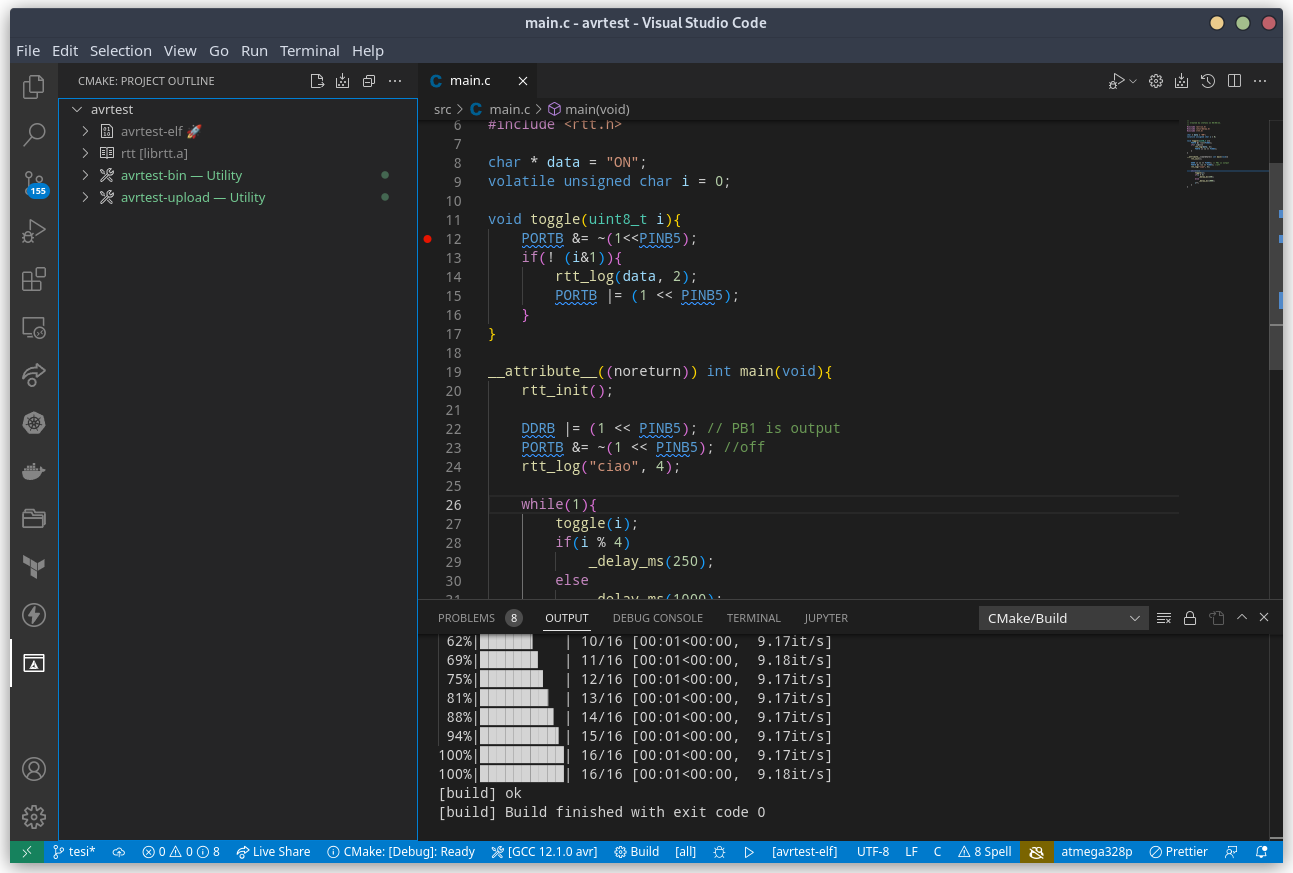
\includegraphics[width=.8\textwidth]{vscode-cmake.png}
    \caption[Immagine del software Visual Studio Code]{Visual Studio Code con il plugin CMake installato}\label{fig:vscode-cmake-plugin}
\end{figure}

Nella figura mostrata è possibile identificare la lista di obiettivi rilevati dal file di configurazione (\texttt{CMakeFile.txt}) come mostrati dalla~\cref{s:cmake}. Nel riquadro presente nella parte inferiore dell'immagine è possibile osservare l'output del comando di caricamento nella memoria flash del target del firmware compilato.

Grazie ad un'altra serie di plugin sviluppata direttamente da Microsoft è possibile implementare il supporto al linguaggio di programmazione integrando anche uno strumento di assistenza alla scrittura del codice con la possibilità di visualizzare suggerimenti inerenti a quanto viene scritto.

È anche possibile configurare l'ambiente di lavoro per l'utilizzo di un linguaggio compilato come Rust\cite{site:avrrust}, grazie all'utilizzo di librerie di astrazione dell'hardware\cite{site:arduino-hal-rust} e il supporto al compilatore avr-gcc.

In quest'ultimo caso il linguaggio e l'infrastruttura della community permette di fare affidamento su svariate librerie disponibili tramite l'utilizzo di un package-manager (\texttt{cargo}\cite{site:cargo-book})

È evidente come l'impiego di un singolo applicativo fortemente utilizzato possa offrire una vastità di scelte inimmaginabile riguardo la composizione del progetto mantenendo costantemente l'utente vicino al proprio \textit{modus operandi} con il quale abitualmente sviluppa software, garantendo elevata efficienza ed ergonomicità.

Osservando la costituzione dell'applicativo più in generale possiamo sottolineare come sia possibile configurare un processo di compilazione personalizzato pur mantenendo la compatibilità con il sistema progettato semplicemente integrando e supportando la possibilità di \textit{debuggare} il codice tramite GDB e avendo gli strumenti necessari per generare un file binario per la programmazione. 

Una volta completata la configurazione è possibile utilizzare le piene potenzialità dell'ambiente di sviluppo integrato come mostrato in~\cref{fig:vscode-debug}.

\begin{figure}
    \centering
    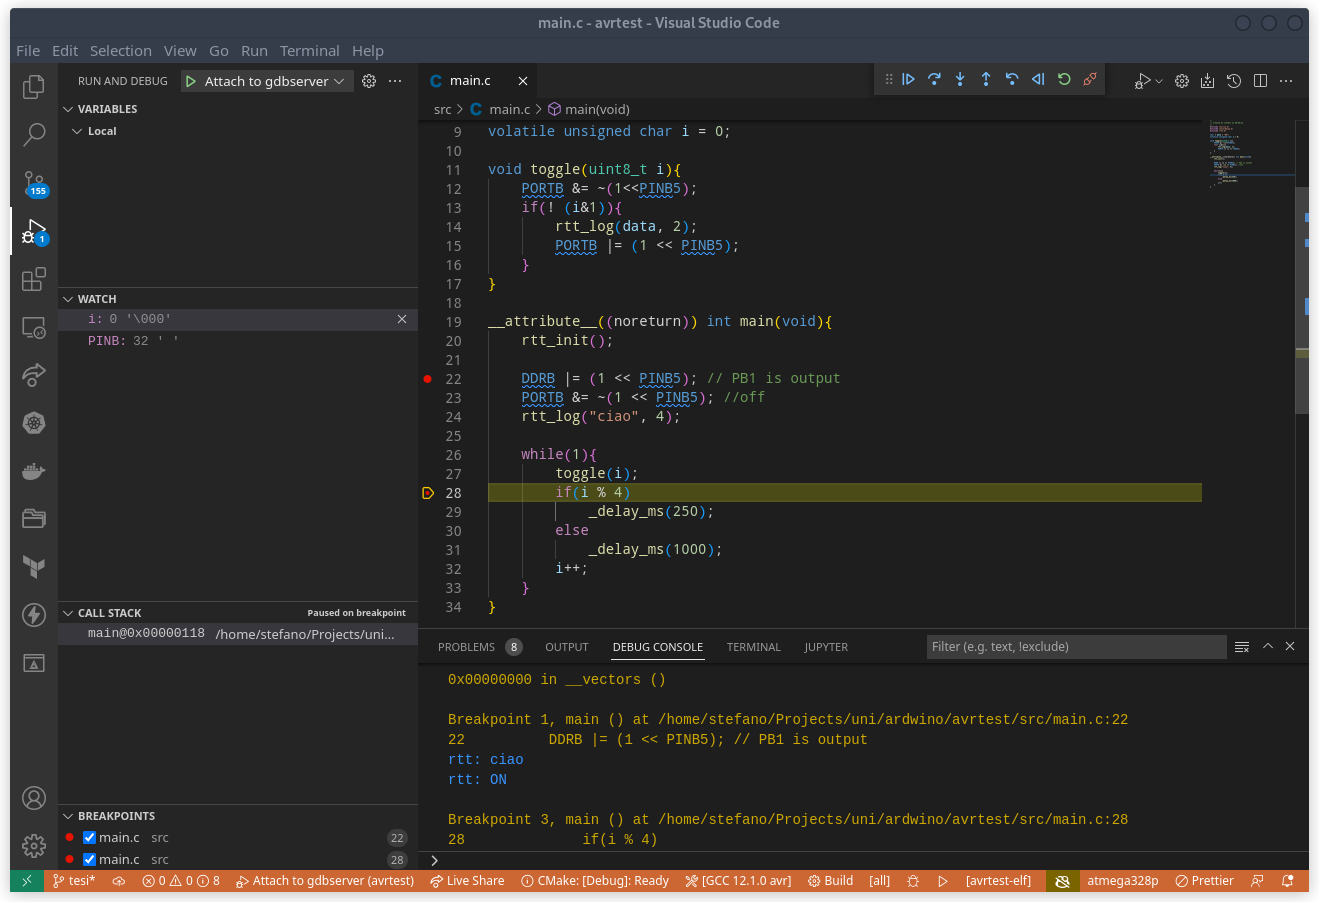
\includegraphics[width=.8\textwidth]{vscode-dbg.png}
    \caption[Immagine del software Visual Studio Code]{Visual Studio Code in modalità di debugging}\label{fig:vscode-debug}
\end{figure}

È possibile osservare come, abilitando il plugin di debug, sia disponibile un riquadro dedicato alla visualizzazione delle informazioni ottenute dal client GDB sul lato sinistro, mentre è identificabile nella parte sottostante l'output del terminale RTT (\cref{s:rtt}) evidenziato in colore blu.

Infine è osservabile la decorazione del codice durante il processo di debug come descritto dalla~\cref{ss:code-decoration}